\PassOptionsToPackage{quiet}{fontspec}  %depress the problem of font
\documentclass[12pt, a4paper, oneside]{ctexart}
\usepackage{amsmath, amsthm, amssymb, bm, graphicx, hyperref, mathrsfs,fontspec}
\setmainfont{Times New Roman}  % 可以写在导言区,也可以写在正文区

\title{\textbf{GitHub使用技巧}}
\author{周雷}
\date{\today}
\linespread{1.3}
\newcounter{problemname}
\newenvironment{problem}{\stepcounter{problemname}\par\noindent\textbf{题目\arabic{problemname}. }}{\\\par}
\newenvironment{solution}{\par\noindent\textbf{解答. }}{\\\par}
\newenvironment{note}{\par\noindent\textbf{题目\arabic{problemname}的注记. }}{\\\par}

\begin{document}

\maketitle

\begin{problem}
    初识Github。
\end{problem}

\begin{solution}
GitHub 是一个面向开源及私有软件项目的托管平台,因为只支持 Git 作为唯一的版本库格式进行托管,故名 GitHub。GitHub 于 2008 年 4 月 10 日正式上线,除了 Git 代码仓库托管及基本的 Web 管理界面以外,还提供了\emph{订阅、讨论组、文本渲染、在线文件编辑器、协作图谱(报表)、代码片段分享(Gist)}等功能。目前,其托管版本数量非常之多,而且其中不乏知名开源项目,例如 Ruby on Rails、jQuery、python 等。

作为开源代码库以及版本控制系统,Github 拥有超过千万的开发者用户。随着越来越多的应用程序转移到了云上,Github 已经成为了管理软件开发以及发现已有代码的首选方法。如前所述,作为一个分布式的版本控制系统,在 Git 中并不存在主库这样的概念,每一份复制出的库都可以独立使用,任何两个库之间的不一致之处都可以进行合并。GitHub 可以托管各种 Git 库,并提供一个 web 界面,但与其它像 SourceForge 或 Google Code 这样的服务不同,GitHub 的独特卖点在于从另外一个项目进行分支的简易性。为一个项目贡献代码非常简单:首先点击项目站点的Fork的按钮,然后将代码检出并将修改加入到刚才分出的代码库中,最后通过内建的pull request机制向项目负责人申请代码合并。GitHub 项目本身自然而然的也在 GitHub 上进行托管,只不过在一个私有的,公共视图不可见的库中。开源项目可以免费托管,但私有库则并非如此。在 GitHub,用户可以通过Explore轻而易举地找到海量的开源代码。因此,称之为程序员的 圣地 也不过吧?
\end{solution}

\begin{problem}
    维护自己的网页
\end{problem}

\begin{solution}
    如果以后我们要在 GitHub 上搭建自己的个人博客,其默认地址就是\href{https://github.com/ZhouLei-maker}{https://github.com/ZhouLei-maker}。GitHub 的仓库分为两种,一种是public repositories公开免费版,一种是private repositories私有付费版。其中,私有仓库一般是由企业或者不希望自己的仓库公开的个人用户购买,这也是 GitHub 的主要收入来源。
\end{solution}

\begin{problem}
    Github文件结构
\end{problem}

\begin{solution}
    包含 3 个commit,第一个 commit 是我们通过勾选Initialize this repository with a README,创建了一个初始化提交文件README.md,其中文件后缀为.md,表示文件为 Markdown 格式;包含 1 个branch,为master分支,即主分支;包含 1 个contributor,为贡献者,也就是我们自己。
\end{solution}

\begin{problem}
    Github常用术语
\end{problem}

\begin{solution}
    Repository:简称Repo,可以理解为“仓库”,我们的项目就存放在仓库之中。也就是说,如果我们想要建立项目,就得先建立仓库;有多个项目,就建立多个仓库。
    
    Issues:可以理解为“问题”,举一个简单的例子,如果我们开源一个项目,如果别人看了我们的项目,并且发现了bug,或者感觉那个地方有待改进,他就可以给我们提出Issue,等我们把Issues解决之后,就可以把这些Issues关闭;反之,我们也可以给他人提出Issue。
    
    Star:可以理解为“点赞”,当我们感觉某一个项目做的比较好之后,就可以为这个项目点赞,而且我们点赞过的项目,都会保存到我们的Star之中,方便我们随时查看。在 GitHub 之中,如果一个项目的点星数能够超百,那么说明这个项目已经很不错了。

Fork:可以理解为“拉分支”,如果我们对某一个项目比较感兴趣,并且想在此基础之上开发新的功能,这时我们就可以Fork这个项目,这表示复制一个完成相同的项目到我们的 GitHub 账号之中,而且独立于原项目。之后,我们就可以在自己复制的项目中进行开发了。

Pull Request:可以理解为“提交请求”,此功能是建立在Fork之上的,如果我们Fork了一个项目,对其进行了修改,而且感觉修改的还不错,我们就可以对原项目的拥有者提出一个Pull请求,等其对我们的请求审核,并且通过审核之后,就可以把我们修改过的内容合并到原项目之中,这时我们就成了该项目的贡献者。

Merge:可以理解为“合并”,如果别人Fork了我们的项目,对其进行了修改,并且提出了Pull请求,这时我们就可以对这个Pull请求进行审核。如果这个Pull请求的内容满足我们的要求,并且跟我们原有的项目没有冲突的话,就可以将其合并到我们的项目之中。当然,是否进行合并,由我们决定。

Watch:可以理解为“观察”,如果我们Watch了一个项目,之后,如果这个项目有了任何更新,我们都会在第一时候收到该项目的更新通知。

Gist:如果我们没有项目可以开源或者只是单纯的想分享一些代码片段的话,我们就可以选择Gist。不过说心里话,如果不翻墙的话,Gist并不好用。
\end{solution}

\begin{problem}
    国内类似的仓库
\end{problem}
\begin{solution}
    \href{https://gitee.com}{https://gitee.com}
    \\账号:18721290631
    \\密码:zhou0624
    \\用户名:ZhouLei\_Maker
    \\绑定邮箱:\href{18240327963@163.com}{18240327963@163.com}
\end{solution}

\begin{problem}
    git操作步骤:
\end{problem}

\begin{solution}
    \begin{itemize}
        \item 首先配置全局变量,主要需要指定用户名和邮箱,可以是虚拟的名称,需要用到的命令为:
        \\git config --global user.name = ‘your name’
        \\git config --global user.email = ‘email address’
        \item 打开要管理的文件夹
        \item 在目标文件夹中打开终端窗口,初始化文件夹,git init,告诉文件夹我要开始管理了
        \item 将文件夹中的文件添加进缓冲区,git add . "."表示将所有文件夹都添加进去,准备发射
        \item 将文件提交到仓库里面, git commit -m "描述",将改好的代码发射到仓库。 
        \item 版本回滚,先使用git log;git rest -hard 版本号。版本号是一串奇怪的字母。
    \end{itemize}
    其他过程和上述步骤一致。
\end{solution}

\begin{problem}
    git用途
\end{problem}
\begin{solution}
    分布式、版本控制、论文写作、软件开发
\end{solution}

\begin{problem}
    GitHub账号密码
\end{problem}
\begin{solution}
    \href{https://github.com/ZhouLei-maker}{https://github.com/ZhouLei-maker}
    \\账号:18240327963@163.com
    \\密码:Zhou0624
    \\用户名:ZhouLei-maker
    \\绑定邮箱:\href{18240327963@163.com}{18240327963@163.com}
\end{solution}

\begin{problem}
    git双向回滚
\end{problem}
\begin{solution}
    work in there + 图片
\end{solution}

\begin{problem}
    git和GitHub协调工作,在多地工作
\end{problem}
\begin{solution}
    case
\end{solution}


% \begin{problem}
%     git和GitHub交互
% \end{problem}
% \begin{solution}
%     git remote add origin \href{https://github.com/ZhouLei-maker/thesis_doctor_latex_template.git}{https://github.com/ZhouLei-maker/thesis_doctor_latex_template.git}
    
% \end{solution}

\begin{problem}
    git和GitHub协调工作流程(单人工作流程)
\end{problem}
\begin{solution}
    \begin{itemize}
        \item 添加远程连接,给GitHub远程仓库起别名,只需要记录一次,使用完该命令可以使用命令 cat .git/config 查看配置信息
        \\git remote add origin <github仓库地址>
        \item 推送代码,一般情况下,将master(主线)的文件推送至GitHub的主线中,将支线文件推送到支线。tips:\emph{推送到支线仓库,本地也要处于支线branch。}例如,master-->master,dev-->dev
        \\git push origin <分支名称>
        \item 下载代码,只有在第一次下载代码时用到。多用于在一个新的本地机器上开始工作时使用。
        \\git clone <github仓库地址>
        \\该命令执行结束之后,自动将该地址映射为origin变量,可以在配置文件中查看。
        \item 更新代码,为了避免复杂,多次clone代码,之后只下载代码的补丁。
        \\git pull origin dev
        \\表示的是拉取远程GitHub仓库中dev分支上的补丁(代码),此时本地分支也应该处于dev分支。此命令也等价于:
        \\git fetch origin dev
        \\git merge origin dev 
        \\本地分支也应该处于dev分支上      
        \item 保持代码提交的整洁性,这一部分内容相对难一点。
        \item 记录整个文件版本过程,包括文字和图形,使用命令:
        \\git log
        \\git log --graph (图形显示,为双短线,latex快捷编译的设置,懒得改了,大部分为双短线,缩写一般是单短线)
        \\git log --graph --pretty=format:"\%h \%s"(简洁显示,只显示不同版本的哈希值和提交备注)       
    \end{itemize}
    上述过程为单人不同地点,不同服务器之间的工作协助流程。
\end{solution}

\begin{problem}
    不同分支之间协作的过程中,文件发生冲突的如何处理?
\end{problem}
\begin{solution}
    使用\emph{Beyond Compare}处理文件冲突问题。两者是不同的两个软件,第一步应该让两个软件关联起来(配置文件)。安装方法直接Google。在git中直接配置一下信息:
    \\git config --local merge.tool bc3
    \\git config --local mergetool.path '/usr/local/bin/bcomp',后面为软件的安装地址。
    \\git config --local mergetool.keepBackup false (不保留备份文件)
    \\git mergetool (运行程序,界面式解决冲突)
    \\local表示只在当前项目文件夹中有效。
\end{solution}

\begin{problem}
    如何给开源代码做贡献,希望扬名立望。
\end{problem}
\begin{solution}
    在GitHub上寻找知名大型的开源软件,发现问题--->解决问题。
    \begin{itemize}
        \item[1] Fork GitHub上知名的代码。Fork过程是将别人远程仓库的代码复制到自己的远程仓库中。
        \item[2] 和前面单人工作流类似,将Fork到自己远程仓库的项目(project) 克隆到本地电脑,在本地电脑上修改调试。
        \item[3] 修改完程序后,将revised的代码push到自己的远程仓库,和自己工作的版本管理过程相同。完成二次开发的项目此时位于自己的远程仓库。
        \item[4] 希望程序发布者看到自己的修改甚至接受自己的修改。\emph{在自己的远程仓库中点击code面板内的“New pull request”选项,将自己仓库中的master提交给源代码的master。点击“Create pull request”。点击之后还可以写一个说明文件,类似于评论。再次点击“Create pull request”。此时源码工作者的目录中会收到一个pull request。如果源码工作者接受,自己的工作就会在源码的提交记录中,如果拒绝,他会直接关闭pull request,或者不做任何评论。}
    \end{itemize}

    希望自己能够做一个默默的大神。
\end{solution}

\begin{problem}
    不同级别的配置文件
\end{problem}
\begin{solution}
    配置文件有三个级别,local、global、system
    \\local只在当前工作目录下有效,称为项目配置文件,位于 项目/.git/config文件中
    \\global全局配置文件,位于 ~/.gitconfig文件中,配置内容,所有git项目都可以通用。
    \\system系统配置文件,位于/etc/.gitconfig文件中.修改需要root权限。

    寻找配置文件的顺序为从上到下。现在本地找,找不到去全局找。一般情况下,远程仓库的地址配置在项目配置文件,姓名邮件配置在全局配置文件中。
\end{solution}

\begin{problem}
    多人协作工作流
\end{problem}
\begin{solution}
    分布式操作
\end{solution}

\begin{problem}
    指定被版本控制的文件及文件夹
\end{problem}
\begin{solution}
    使用\emph{.gitignore}文件。如何设置文件及文件夹可以可以百度,参考其语法。
\end{solution}

\begin{problem}
    Issues、Wiki的使用方法
\end{problem}
\begin{solution}
    wiki里面可以写项目的简介,备注项目相关的信息。类似于说明书。

    Issue可以对项目提出问题,该问题可以指向某个具体的人,别人可以来回答。保证该问题不会被重复问到。第二个功能是bug管理。说明bug,指向某个人,指派任务让他来解决。也可以查看任务的状态,选择关闭和开放。
\end{solution}

\begin{problem}
    免密登陆
\end{problem}
\begin{solution}
    使用\emph{gh}软件。百度结果随处都是。其中会用到\emph{token}密钥。
\end{solution}

\begin{problem}
    rebase(变基)的用法
\end{problem}
\begin{solution}
    作用:使git记录简洁。(多个记录整合为一个记录)语法如下:

    git rebase -i HEAD~3 将三条记录合并成一个。合并记录时尽量不要和已经push到仓库的版本合并。只在本地合并。

    版本控制过程中,分支的合并,用来取消rebase。用来将分支结构放在master(主干)上。分为三步:
    \newline  git checkout dev      切换到分支上
    \newline  git rebase master     在分支上rebase主干master
    \newline  git checkout master       切换到master
    \newline  git merge dev         将分支dev合并到master

    这样显示的结果是一条主干线,没有分叉。
\end{solution}

\begin{problem}
    有一种情况:代码放在云端,周雷在办公室写了一段代码,忘记上传在GitHub,回到宿舍,突发奇想,想写代码,只能在办公室代码前一个版本上进行继续工作,工作完成之后上传至github。第二天到公司打开电脑,拉代码时,会出现分支,会有变基提醒。这种情况也发生在多人协助完成一个项目时。
\end{problem}
\begin{solution}
    第二天在公司拉代码时会进行一次合并。出现分叉的情况。git pull 会产生分叉。git pull 命令相当于git fetch + git merge。本质上是merge出现分支,解决这个问题,可以用rebase命令。命令如下:git fetch origin dev; git rebase origin/dev。
\end{solution}
\begin{note}
    操作中可能出现冲突,git rebase 会显示冲突,根据提示,输入代码,再输入git rebase --continue,表示继续rebase。
\end{note}

\begin{problem}
    git push -u origin master
    \newline
    git commit -m "description"
    \\其中u,m的含义。
\end{problem} 
\begin{solution}
    i don't know.第一条push指令中,最后的master,指的是本地的分支。本地的分支。本地的分支。
\end{solution}

\begin{problem}
    远程仓库修改如何同步到本地文件夹?
\end{problem} 
\begin{solution}
    有时候,我们会直接在GitHub上修改文件,多发生在修改说明文档。添加、删除或者减少,此时使用git pull origin master 命令可以直接将网页端的修改拉取下来,在git log 中也可以查出来网页端的commit记录。
\end{solution}

\begin{figure}
    \centering
    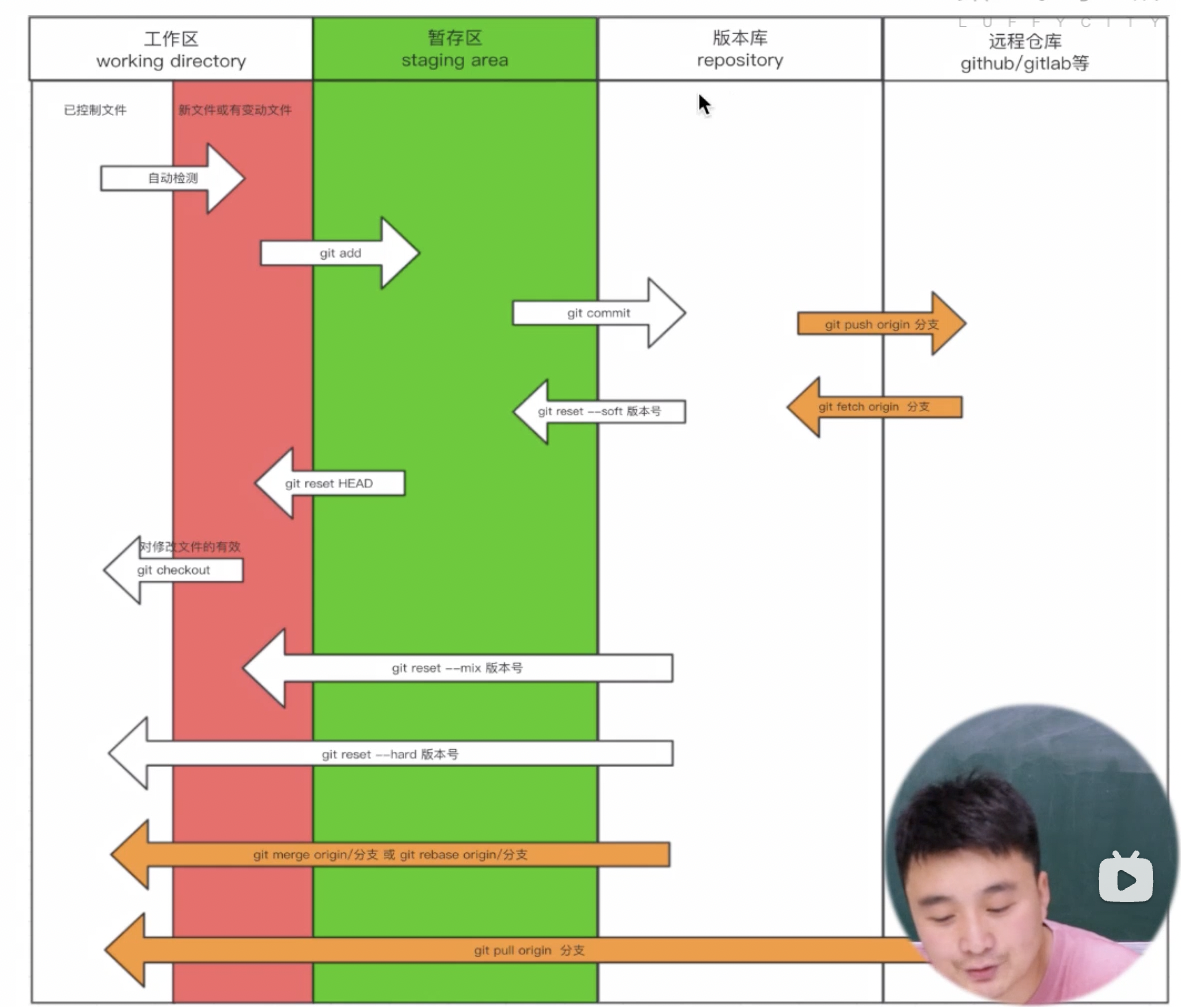
\includegraphics[width = 0.6 \textwidth]{git命令说明图.png}
\end{figure}
\end{document}